\iffalse
	\begin{figure}[H]
		\centering
 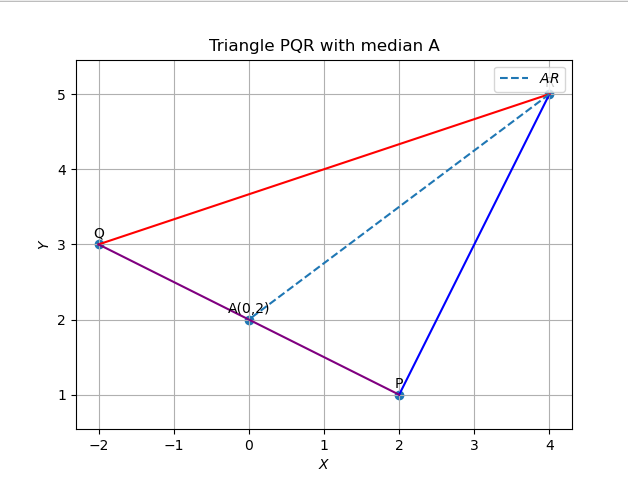
\includegraphics[width=0.75\columnwidth]{chapters/11/10/2/9/figs/line.png}
		\caption{}
		\label{fig:11/10/2/9}
  	\end{figure}
	See Fig. 
		\ref{fig:11/10/2/9}.
		\fi
Using section formula, the mid point of $PQ$ is
\begin{align}
\vec{A} = \frac{\vec{P} +\vec{Q} }{2}
	= {\myvec{0\\2}}
\end{align} 
Following the approach in \probref{chapters/11/10/2/7},
\begin{align*}
	\augvec{2}{1}{ 
	4 & 5 & 1
	\\  
	0 & 2 & 1
	}
	\xleftrightarrow[R_2 \leftarrow 4R_2 ]{R_1 \leftarrow 2R_1 -5R_2}
	\augvec{2}{1}{ 
	8 & 0 & -3 
	\\ 
	0 & 8 & 4 
	}
	\implies \vec{n} = \frac{1}{8}\myvec{ -3 \\ 4}
\end{align*}
Thus,
the equation of the line is 
\begin{align}
	\myvec{-3 & 4}\vec{x} =8 
\end{align}
